Let $\vec{O} = \myvec{0\\0}$ be the intersection point of the diagonals of the rhombus. 
The diagonals of a rhombus bisect one another at right angles. Hence, 
\begin{align}
    \vec{B} = \myvec{2.8\\0}\\
    \vec{E} = \myvec{0\\-3.25}\\
    \vec{N} = \myvec{-2.8\\0}\\
    \vec{D} = \myvec{0\\3.25}
\end{align}
See Fig. \ref{rhombus/aug/2/6}.
\begin{figure}[!ht]
 \centering
 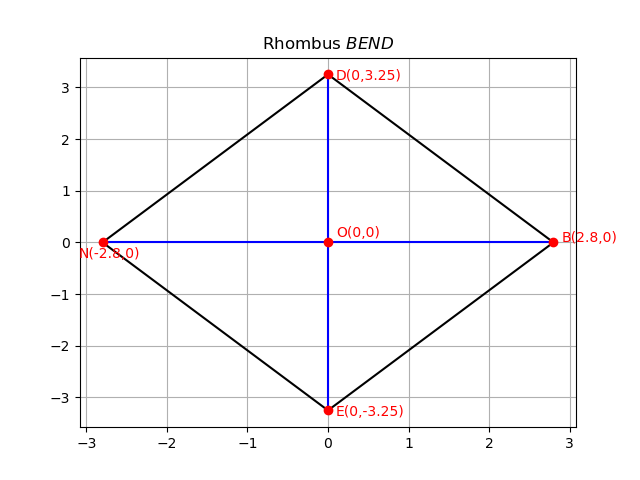
\includegraphics[width=\columnwidth]{solutions/aug/2/6/rhombus_BEND.png}
 \caption{Rhombus $BEND$}
 \label{rhombus/aug/2/6}
 \end{figure}



